% Options for packages loaded elsewhere
% Options for packages loaded elsewhere
\PassOptionsToPackage{unicode}{hyperref}
\PassOptionsToPackage{hyphens}{url}
\PassOptionsToPackage{dvipsnames,svgnames,x11names}{xcolor}
%
\documentclass[
  letterpaper,
  DIV=11,
  numbers=noendperiod]{scrartcl}
\usepackage{xcolor}
\usepackage{amsmath,amssymb}
\setcounter{secnumdepth}{5}
\usepackage{iftex}
\ifPDFTeX
  \usepackage[T1]{fontenc}
  \usepackage[utf8]{inputenc}
  \usepackage{textcomp} % provide euro and other symbols
\else % if luatex or xetex
  \usepackage{unicode-math} % this also loads fontspec
  \defaultfontfeatures{Scale=MatchLowercase}
  \defaultfontfeatures[\rmfamily]{Ligatures=TeX,Scale=1}
\fi
\usepackage{lmodern}
\ifPDFTeX\else
  % xetex/luatex font selection
\fi
% Use upquote if available, for straight quotes in verbatim environments
\IfFileExists{upquote.sty}{\usepackage{upquote}}{}
\IfFileExists{microtype.sty}{% use microtype if available
  \usepackage[]{microtype}
  \UseMicrotypeSet[protrusion]{basicmath} % disable protrusion for tt fonts
}{}
\makeatletter
\@ifundefined{KOMAClassName}{% if non-KOMA class
  \IfFileExists{parskip.sty}{%
    \usepackage{parskip}
  }{% else
    \setlength{\parindent}{0pt}
    \setlength{\parskip}{6pt plus 2pt minus 1pt}}
}{% if KOMA class
  \KOMAoptions{parskip=half}}
\makeatother
% Make \paragraph and \subparagraph free-standing
\makeatletter
\ifx\paragraph\undefined\else
  \let\oldparagraph\paragraph
  \renewcommand{\paragraph}{
    \@ifstar
      \xxxParagraphStar
      \xxxParagraphNoStar
  }
  \newcommand{\xxxParagraphStar}[1]{\oldparagraph*{#1}\mbox{}}
  \newcommand{\xxxParagraphNoStar}[1]{\oldparagraph{#1}\mbox{}}
\fi
\ifx\subparagraph\undefined\else
  \let\oldsubparagraph\subparagraph
  \renewcommand{\subparagraph}{
    \@ifstar
      \xxxSubParagraphStar
      \xxxSubParagraphNoStar
  }
  \newcommand{\xxxSubParagraphStar}[1]{\oldsubparagraph*{#1}\mbox{}}
  \newcommand{\xxxSubParagraphNoStar}[1]{\oldsubparagraph{#1}\mbox{}}
\fi
\makeatother

\usepackage{color}
\usepackage{fancyvrb}
\newcommand{\VerbBar}{|}
\newcommand{\VERB}{\Verb[commandchars=\\\{\}]}
\DefineVerbatimEnvironment{Highlighting}{Verbatim}{commandchars=\\\{\}}
% Add ',fontsize=\small' for more characters per line
\usepackage{framed}
\definecolor{shadecolor}{RGB}{241,243,245}
\newenvironment{Shaded}{\begin{snugshade}}{\end{snugshade}}
\newcommand{\AlertTok}[1]{\textcolor[rgb]{0.68,0.00,0.00}{#1}}
\newcommand{\AnnotationTok}[1]{\textcolor[rgb]{0.37,0.37,0.37}{#1}}
\newcommand{\AttributeTok}[1]{\textcolor[rgb]{0.40,0.45,0.13}{#1}}
\newcommand{\BaseNTok}[1]{\textcolor[rgb]{0.68,0.00,0.00}{#1}}
\newcommand{\BuiltInTok}[1]{\textcolor[rgb]{0.00,0.23,0.31}{#1}}
\newcommand{\CharTok}[1]{\textcolor[rgb]{0.13,0.47,0.30}{#1}}
\newcommand{\CommentTok}[1]{\textcolor[rgb]{0.37,0.37,0.37}{#1}}
\newcommand{\CommentVarTok}[1]{\textcolor[rgb]{0.37,0.37,0.37}{\textit{#1}}}
\newcommand{\ConstantTok}[1]{\textcolor[rgb]{0.56,0.35,0.01}{#1}}
\newcommand{\ControlFlowTok}[1]{\textcolor[rgb]{0.00,0.23,0.31}{\textbf{#1}}}
\newcommand{\DataTypeTok}[1]{\textcolor[rgb]{0.68,0.00,0.00}{#1}}
\newcommand{\DecValTok}[1]{\textcolor[rgb]{0.68,0.00,0.00}{#1}}
\newcommand{\DocumentationTok}[1]{\textcolor[rgb]{0.37,0.37,0.37}{\textit{#1}}}
\newcommand{\ErrorTok}[1]{\textcolor[rgb]{0.68,0.00,0.00}{#1}}
\newcommand{\ExtensionTok}[1]{\textcolor[rgb]{0.00,0.23,0.31}{#1}}
\newcommand{\FloatTok}[1]{\textcolor[rgb]{0.68,0.00,0.00}{#1}}
\newcommand{\FunctionTok}[1]{\textcolor[rgb]{0.28,0.35,0.67}{#1}}
\newcommand{\ImportTok}[1]{\textcolor[rgb]{0.00,0.46,0.62}{#1}}
\newcommand{\InformationTok}[1]{\textcolor[rgb]{0.37,0.37,0.37}{#1}}
\newcommand{\KeywordTok}[1]{\textcolor[rgb]{0.00,0.23,0.31}{\textbf{#1}}}
\newcommand{\NormalTok}[1]{\textcolor[rgb]{0.00,0.23,0.31}{#1}}
\newcommand{\OperatorTok}[1]{\textcolor[rgb]{0.37,0.37,0.37}{#1}}
\newcommand{\OtherTok}[1]{\textcolor[rgb]{0.00,0.23,0.31}{#1}}
\newcommand{\PreprocessorTok}[1]{\textcolor[rgb]{0.68,0.00,0.00}{#1}}
\newcommand{\RegionMarkerTok}[1]{\textcolor[rgb]{0.00,0.23,0.31}{#1}}
\newcommand{\SpecialCharTok}[1]{\textcolor[rgb]{0.37,0.37,0.37}{#1}}
\newcommand{\SpecialStringTok}[1]{\textcolor[rgb]{0.13,0.47,0.30}{#1}}
\newcommand{\StringTok}[1]{\textcolor[rgb]{0.13,0.47,0.30}{#1}}
\newcommand{\VariableTok}[1]{\textcolor[rgb]{0.07,0.07,0.07}{#1}}
\newcommand{\VerbatimStringTok}[1]{\textcolor[rgb]{0.13,0.47,0.30}{#1}}
\newcommand{\WarningTok}[1]{\textcolor[rgb]{0.37,0.37,0.37}{\textit{#1}}}

\usepackage{longtable,booktabs,array}
\usepackage{calc} % for calculating minipage widths
% Correct order of tables after \paragraph or \subparagraph
\usepackage{etoolbox}
\makeatletter
\patchcmd\longtable{\par}{\if@noskipsec\mbox{}\fi\par}{}{}
\makeatother
% Allow footnotes in longtable head/foot
\IfFileExists{footnotehyper.sty}{\usepackage{footnotehyper}}{\usepackage{footnote}}
\makesavenoteenv{longtable}
\usepackage{graphicx}
\makeatletter
\newsavebox\pandoc@box
\newcommand*\pandocbounded[1]{% scales image to fit in text height/width
  \sbox\pandoc@box{#1}%
  \Gscale@div\@tempa{\textheight}{\dimexpr\ht\pandoc@box+\dp\pandoc@box\relax}%
  \Gscale@div\@tempb{\linewidth}{\wd\pandoc@box}%
  \ifdim\@tempb\p@<\@tempa\p@\let\@tempa\@tempb\fi% select the smaller of both
  \ifdim\@tempa\p@<\p@\scalebox{\@tempa}{\usebox\pandoc@box}%
  \else\usebox{\pandoc@box}%
  \fi%
}
% Set default figure placement to htbp
\def\fps@figure{htbp}
\makeatother





\setlength{\emergencystretch}{3em} % prevent overfull lines

\providecommand{\tightlist}{%
  \setlength{\itemsep}{0pt}\setlength{\parskip}{0pt}}



 
\usepackage[]{biblatex}


\KOMAoption{captions}{tableheading}
\makeatletter
\@ifpackageloaded{caption}{}{\usepackage{caption}}
\AtBeginDocument{%
\ifdefined\contentsname
  \renewcommand*\contentsname{Table of contents}
\else
  \newcommand\contentsname{Table of contents}
\fi
\ifdefined\listfigurename
  \renewcommand*\listfigurename{List of Figures}
\else
  \newcommand\listfigurename{List of Figures}
\fi
\ifdefined\listtablename
  \renewcommand*\listtablename{List of Tables}
\else
  \newcommand\listtablename{List of Tables}
\fi
\ifdefined\figurename
  \renewcommand*\figurename{Figure}
\else
  \newcommand\figurename{Figure}
\fi
\ifdefined\tablename
  \renewcommand*\tablename{Table}
\else
  \newcommand\tablename{Table}
\fi
}
\@ifpackageloaded{float}{}{\usepackage{float}}
\floatstyle{ruled}
\@ifundefined{c@chapter}{\newfloat{codelisting}{h}{lop}}{\newfloat{codelisting}{h}{lop}[chapter]}
\floatname{codelisting}{Listing}
\newcommand*\listoflistings{\listof{codelisting}{List of Listings}}
\makeatother
\makeatletter
\makeatother
\makeatletter
\@ifpackageloaded{caption}{}{\usepackage{caption}}
\@ifpackageloaded{subcaption}{}{\usepackage{subcaption}}
\makeatother
\usepackage{bookmark}
\IfFileExists{xurl.sty}{\usepackage{xurl}}{} % add URL line breaks if available
\urlstyle{same}
\hypersetup{
  pdftitle={Manifesto Text Clustering},
  colorlinks=true,
  linkcolor={blue},
  filecolor={Maroon},
  citecolor={Blue},
  urlcolor={Blue},
  pdfcreator={LaTeX via pandoc}}


\title{Manifesto Text Clustering}
\author{}
\date{}
\begin{document}
\maketitle

\renewcommand*\contentsname{Table of contents}
{
\hypersetup{linkcolor=}
\setcounter{tocdepth}{3}
\tableofcontents
}

\section{Data}\label{data}

This project utilizes data from the
\href{https://manifesto-project.wzb.eu/}{Comparative Manifesto Project
(CMP)}, which provides political manifestos annotated at the
quasi-sentence level. These annotations include manually assigned policy
codes corresponding to predefined political topics. The objective of
this project is to use the text content of these
quasi-sentences---without labels---to cluster them into coherent topic
groups resembling the CMP's main categories.

\subsection{Data Source and Access}\label{data-source-and-access}

The data is accessed programmatically via the CMP's official REST API.
An API key is used for authenticated requests. Using a series of
endpoint queries, the following resources were retrieved:

\begin{itemize}
\tightlist
\item
  \textbf{Core dataset metadata} (party, country, date, etc.)
\item
  \textbf{Manifesto metadata} to filter for English translations and
  machine-readable annotations
\item
  \textbf{Full quasi-sentence text} and their respective structure for
  selected manifestos
\end{itemize}

Data retrieval is restricted to manifestos from Germany, Switzerland,
and Austria, where English translations and machine-annotated versions
are available.

\subsection{Manifesto Selection
Criteria}\label{manifesto-selection-criteria}

From the full list of manifestos, only a subset was selected based on
the following conditions:

\begin{enumerate}
\def\labelenumi{\arabic{enumi}.}
\tightlist
\item
  Country must be Germany, Switzerland, or Austria
\item
  Manifesto must have an English translation
  (\texttt{translation\_en\ =\ True})
\item
  Manifesto must include sentence-level annotations
  (\texttt{annotations\ =\ True})
\item
  Only the latest manifesto per party is kept to avoid duplication and
  ensure contemporary relevance
\end{enumerate}

\begin{verbatim}
Daten aus Cache geladen.
\end{verbatim}

\subsection{Quasi-Sentence Extraction}\label{quasi-sentence-extraction}

The text content of each manifesto is returned as a list of
quasi-sentences---units of meaning used by CMP to annotate policy
content. These were extracted and aggregated into a dictionary of the
form:

\begin{Shaded}
\begin{Highlighting}[]
\NormalTok{\{}
    \StringTok{"manifesto\_id\_1"}\NormalTok{: [}
\NormalTok{        \{}\StringTok{"text"}\NormalTok{: }\StringTok{"qs1"}\NormalTok{, }\StringTok{"cmp\_code"}\NormalTok{: }\DecValTok{101}\NormalTok{\},}
\NormalTok{        \{}\StringTok{"text"}\NormalTok{: }\StringTok{"qs2"}\NormalTok{, }\StringTok{"cmp\_code"}\NormalTok{: }\DecValTok{204}\NormalTok{\},}
\NormalTok{        \{}\StringTok{"text"}\NormalTok{: }\StringTok{"qs3"}\NormalTok{, }\StringTok{"cmp\_code"}\NormalTok{: }\DecValTok{503}\NormalTok{\},}
        \CommentTok{\# ...}
\NormalTok{    ],}
    \StringTok{"manifesto\_id\_2"}\NormalTok{: [}
\NormalTok{        \{}\StringTok{"text"}\NormalTok{: }\StringTok{"qs1"}\NormalTok{, }\StringTok{"cmp\_code"}\NormalTok{: }\DecValTok{402}\NormalTok{\},}
\NormalTok{        \{}\StringTok{"text"}\NormalTok{: }\StringTok{"qs2"}\NormalTok{, }\StringTok{"cmp\_code"}\NormalTok{: }\DecValTok{302}\NormalTok{\},}
        \CommentTok{\# ...}
\NormalTok{    ],}
    \CommentTok{\# ...}
\NormalTok{\}}
\end{Highlighting}
\end{Shaded}

\subsection{Category Mapping}\label{category-mapping}

lthough this is an unsupervised task, the CMP codebook was downloaded
and consulted to define reference categories for qualitative evaluation.
The seven CMP ``main domains'' used as reference topics are:

\begin{enumerate}
\def\labelenumi{\arabic{enumi}.}
\tightlist
\item
  External Relations
\item
  Freedom and Democracy
\item
  Political System
\item
  Economy
\item
  Welfare and Quality of Life
\item
  Fabric of Society
\item
  Social Groups
\end{enumerate}

These categories serve as a qualitative benchmark to interpret the
discovered clusters. While these are not used directly in training or
clustering, several hand-coded samples are referenced for evaluation in
Section 4.

The resulting dataframe looks like this:

\begin{longtable}[]{@{}
  >{\raggedright\arraybackslash}p{(\linewidth - 6\tabcolsep) * \real{0.1892}}
  >{\raggedright\arraybackslash}p{(\linewidth - 6\tabcolsep) * \real{0.3514}}
  >{\raggedright\arraybackslash}p{(\linewidth - 6\tabcolsep) * \real{0.1351}}
  >{\raggedright\arraybackslash}p{(\linewidth - 6\tabcolsep) * \real{0.3243}}@{}}
\toprule\noalign{}
\begin{minipage}[b]{\linewidth}\raggedright
manifesto\_id
\end{minipage} & \begin{minipage}[b]{\linewidth}\raggedright
text
\end{minipage} & \begin{minipage}[b]{\linewidth}\raggedright
cmp\_code
\end{minipage} & \begin{minipage}[b]{\linewidth}\raggedright
category
\end{minipage} \\
\midrule\noalign{}
\endhead
\bottomrule\noalign{}
\endlastfoot
GER\_202109 & ``We support\ldots{}'' & 403 & Economy \\
GER\_202109 & ``Democracy is essential'' & 201 & Freedom and
Democracy \\
\end{longtable}

\subsection{Data Exploration}\label{data-exploration}

First, I explore the Data in the form described previously to get an
idea if it is ready for clustering or if it needs pore preprocessing.

\begin{verbatim}
Number of quasi-sentences: 36088
Number of unique manifestos: 34
Number of unique categories: 7
\end{verbatim}

\pandocbounded{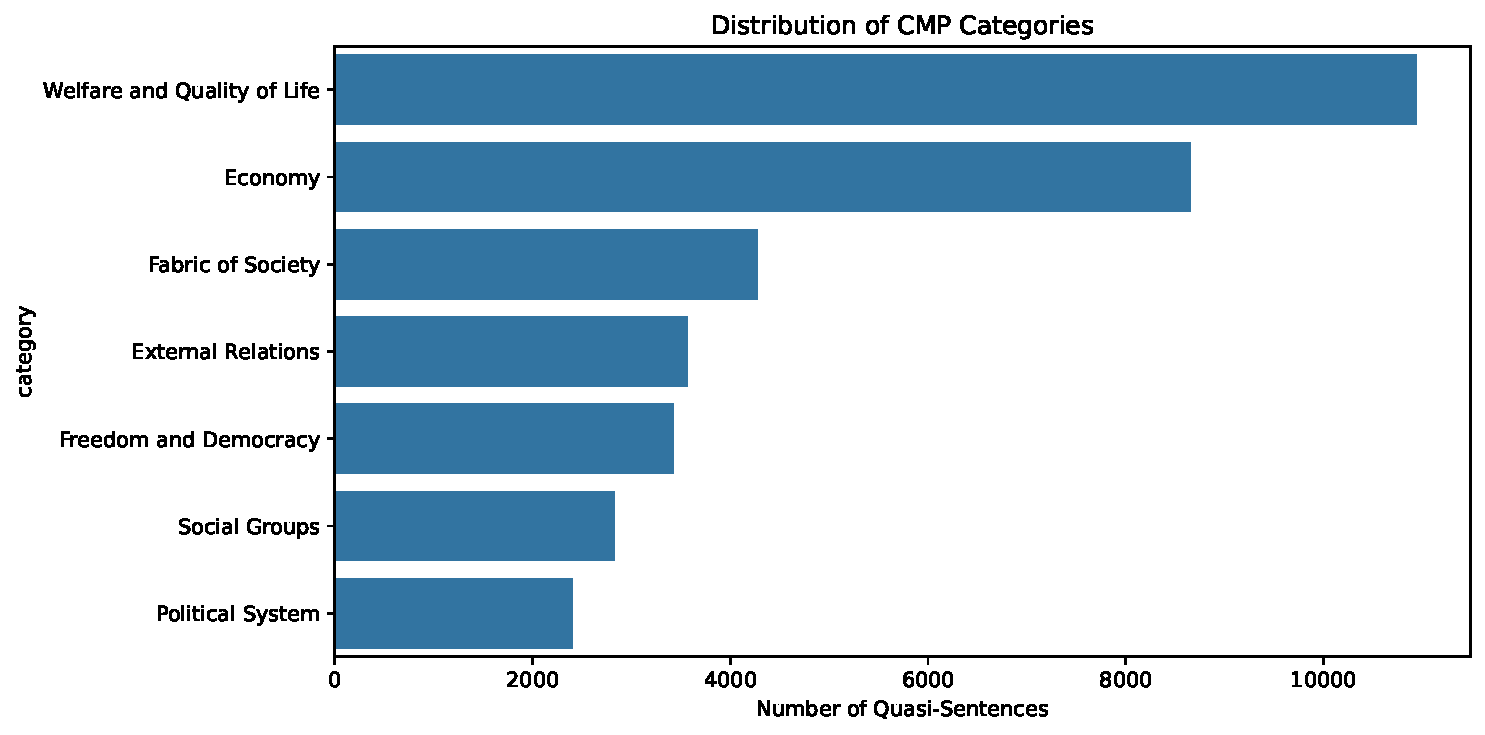
\includegraphics[keepaspectratio]{manifesto_text_clustering_files/figure-pdf/cell-8-output-1.pdf}}

\pandocbounded{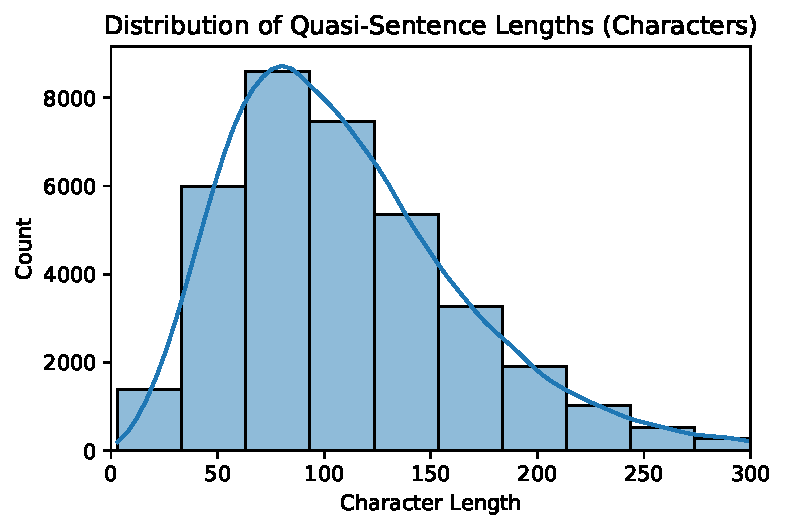
\includegraphics[keepaspectratio]{manifesto_text_clustering_files/figure-pdf/cell-9-output-1.pdf}}

\pandocbounded{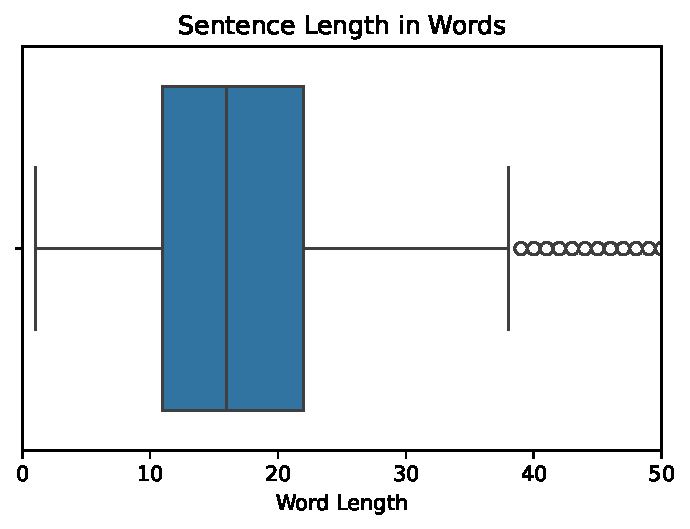
\includegraphics[keepaspectratio]{manifesto_text_clustering_files/figure-pdf/cell-10-output-1.pdf}}

To get an idea about the content of the categories, I take a look at the
most frequent words. Here I take the example of Economy.

\pandocbounded{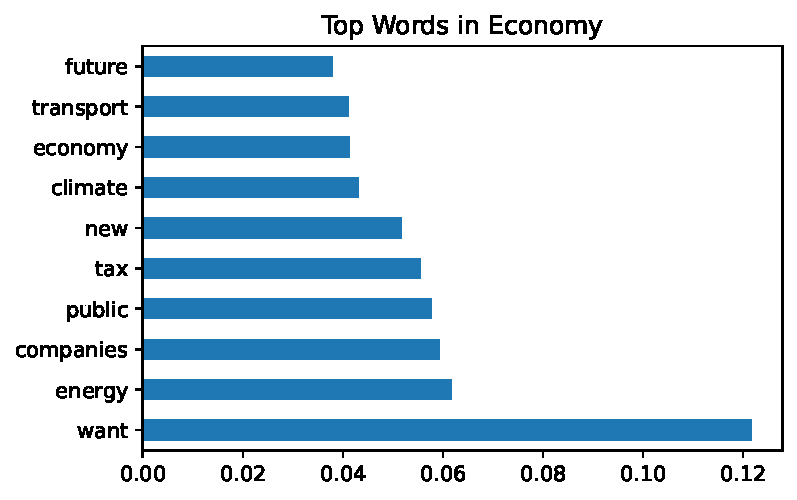
\includegraphics[keepaspectratio]{manifesto_text_clustering_files/figure-pdf/cell-11-output-1.pdf}}

\subsection{Grouping Sentences}\label{grouping-sentences}

In the Data Exploration Step I realized that the length of the
Quasi-Sentences would be a problem. The average length is only about
fifteen words which makes the Clustering Task very difficult until
almost impossible. For this reason the Quasi-Sentences are grouped to
perform the Machine Learning Task as Follows.

\begin{longtable}[]{@{}
  >{\raggedright\arraybackslash}p{(\linewidth - 8\tabcolsep) * \real{0.1573}}
  >{\raggedright\arraybackslash}p{(\linewidth - 8\tabcolsep) * \real{0.2921}}
  >{\raggedright\arraybackslash}p{(\linewidth - 8\tabcolsep) * \real{0.1124}}
  >{\raggedright\arraybackslash}p{(\linewidth - 8\tabcolsep) * \real{0.2697}}
  >{\raggedright\arraybackslash}p{(\linewidth - 8\tabcolsep) * \real{0.1685}}@{}}
\toprule\noalign{}
\begin{minipage}[b]{\linewidth}\raggedright
manifesto\_id
\end{minipage} & \begin{minipage}[b]{\linewidth}\raggedright
text
\end{minipage} & \begin{minipage}[b]{\linewidth}\raggedright
cmp\_code
\end{minipage} & \begin{minipage}[b]{\linewidth}\raggedright
category
\end{minipage} & \begin{minipage}[b]{\linewidth}\raggedright
sentence\_group
\end{minipage} \\
\midrule\noalign{}
\endhead
\bottomrule\noalign{}
\endlastfoot
GER\_202109 & ``We support\ldots{}'' & 403.1 & Economy & 1 \\
GER\_202109 & ``\ldots are taxes\ldots{}'' & 403.2 & Economy & 1 \\
GER\_202109 & ``Democracy is essential'' & 201 & Freedom and Democracy &
2 \\
\end{longtable}

After Grouping, the distribution of Character Lengths is checked again.
The longer text length should make the Dimensionality Reduction and
Clustering easier.

Each quasi-sentence group was then prepared for embedding using a
sentence-transformer model in the next stage of the pipeline (described
in Section 3).

\begin{verbatim}
   manifesto_id               category  \
0  41113_202109                Economy   
1  41113_202109     External Relations   
2  41113_202109      Fabric of Society   
3  41113_202109  Freedom and Democracy   
4  41113_202109       Political System   

                                                text  
0  Through science and progress. We have seen how...  
1  We have learned how limited national answers t...  
2  It has shown in a good way the commonality, in...  
3  Dear voters, it is through elections that a so...  
4  We, BÜNDNIS 90/DIE GRÜNEN, are presenting our ...  
\end{verbatim}

\subsection{Data Exploration of Sentence
Groups}\label{data-exploration-of-sentence-groups}

\pandocbounded{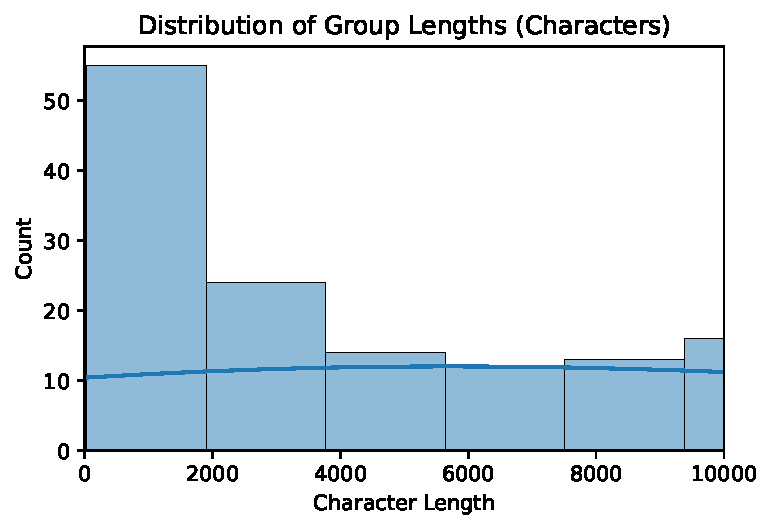
\includegraphics[keepaspectratio]{manifesto_text_clustering_files/figure-pdf/cell-13-output-1.pdf}}

\pandocbounded{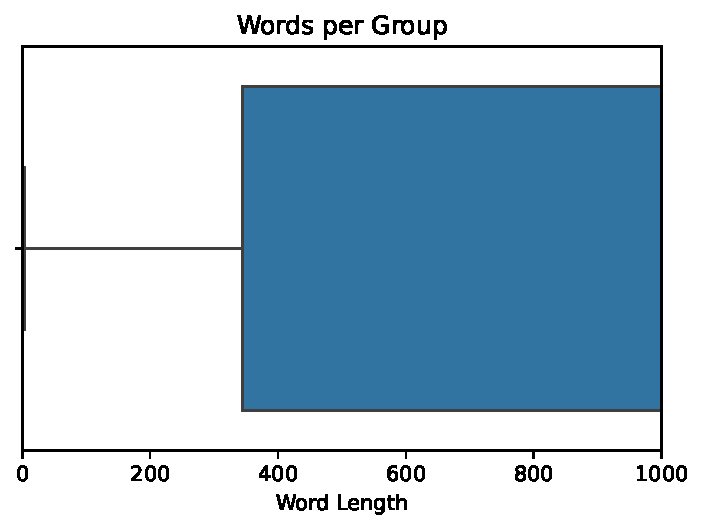
\includegraphics[keepaspectratio]{manifesto_text_clustering_files/figure-pdf/cell-14-output-1.pdf}}

\section{Methods}\label{methods}

The central aim of this project is to cluster quasi-sentences from
political manifestos into coherent topic groups, ideally resembling the
seven high-level categories defined by the Comparative Manifesto Project
(CMP). Since no sentence-level topic labels are used during model
training, the task is unsupervised in nature.

This section describes and motivates the methods used at each stage:
transforming raw text into a numerical representation, reducing
dimensionality for visualization and noise reduction, and applying
clustering algorithms to identify topic-like groupings. Special
attention is given to the suitability of each technique for short
political text fragments and the challenges inherent to topic modeling
without supervision.

\subsection{Sentence Embedding}\label{sentence-embedding}

Quasi-sentences from manifestos are typically short---often no more than
a clause or single policy statement. To represent these as inputs for
clustering, the project uses \emph{sentence embeddings}, which map each
sentence to a fixed-length vector in a high-dimensional space.

The selected model is \textbf{Sentence-BERT (SBERT)}, a
transformer-based architecture specifically designed for semantically
meaningful sentence embeddings. Unlike vanilla BERT, which isn't
optimized for sentence-level similarity, SBERT introduces a siamese
network structure that enables efficient semantic similarity
computation. The pre-trained model \texttt{all-MiniLM-L6-v2} was chosen
for its balance between performance and speed.

Sentence embeddings are preferred over traditional bag-of-words or
TF-IDF vectors for several reasons:

\begin{itemize}
\tightlist
\item
  They capture \textbf{semantic similarity}, not just token overlap.
\item
  They produce \textbf{fixed-size dense vectors}, suitable for
  distance-based clustering.
\item
  They perform well on short, syntactically diverse texts such as
  political quasi-sentences.
\end{itemize}

Each quasi-sentence is thus encoded into a 384-dimensional vector, which
serves as the input to subsequent analysis.

\subsection{Dimensionality Reduction}\label{dimensionality-reduction}

Before applying clustering algorithms, the embedding space is optionally
reduced to a lower dimension to address two issues:

\begin{itemize}
\tightlist
\item
  \textbf{Curse of dimensionality}: In high-dimensional spaces, distance
  metrics become less meaningful, which can degrade clustering
  performance.
\item
  \textbf{Visualization}: Human interpretation of cluster structure
  requires 2D or 3D projections.
\end{itemize}

The method of choice is \textbf{Principal Component Analysis (PCA)}. PCA
projects the data onto a lower-dimensional orthogonal subspace that
captures as much variance as possible. In this project, PCA is used
primarily for:

\begin{itemize}
\tightlist
\item
  Reducing noise in the input to clustering
\item
  Projecting cluster centroids for manual inspection
\item
  Identifying dominant axes of variation across quasi-sentences (e.g.,
  economy vs.~welfare focus)
\end{itemize}

PCA is chosen over nonlinear methods such as t-SNE or UMAP because:

\begin{itemize}
\tightlist
\item
  It is \textbf{deterministic} and interpretable.
\item
  It preserves \textbf{global structure} better, which is useful for
  clustering.
\item
  It enables visualization of loadings (important features) via
  \textbf{biplots}.
\end{itemize}

\subsection{Clustering Algorithms}\label{clustering-algorithms}

\subsubsection{K-Means Clustering}\label{k-means-clustering}

The first method applied is \textbf{k-means clustering}, a
centroid-based algorithm that partitions the data into \emph{k} clusters
by minimizing intra-cluster variance. The objective function is:

\[
\underset{C}{\text{argmin}} \sum_{i=1}^{k} \sum_{\mathbf{x}_j \in C_i} \|\mathbf{x}_j - \boldsymbol{\mu}_i\|^2
\]

where \(\boldsymbol{\mu}_i\) is the centroid of cluster \(C_1\).

K-means is a natural choice because:

\begin{itemize}
\tightlist
\item
  It scales efficiently to large datasets.
\item
  It provides \textbf{hard assignments} (each sentence belongs to
  exactly one cluster).
\item
  It requires minimal assumptions about data distribution.
\end{itemize}

However, k-means has notable limitations:

\begin{itemize}
\tightlist
\item
  It assumes \textbf{spherical clusters of similar size}, which may not
  hold for natural language data.
\item
  It is sensitive to initialization and the chosen number of clusters
  \emph{k}.
\end{itemize}

To mitigate this, the \textbf{elbow method} and \textbf{silhouette
scores} are used to identify a suitable value for \emph{k}, with \emph{k
= 7} being a theoretically motivated target corresponding to the CMP
categories.

\subsubsection{Hierarchical Agglomerative
Clustering}\label{hierarchical-agglomerative-clustering}

To complement k-means, \textbf{hierarchical agglomerative clustering
(HAC)} is applied. HAC recursively merges the most similar clusters
based on a linkage criterion until all data points are grouped into one
hierarchy (a dendrogram). The project uses \textbf{Ward's method}, which
minimizes the increase in total within-cluster variance when merging
clusters.

HAC offers several advantages in this context:

\begin{itemize}
\tightlist
\item
  It does not require pre-specifying the number of clusters.
\item
  It can reveal \textbf{nested structure}, which is conceptually useful
  since some CMP topics (e.g., Economy and Welfare) may be subtopics of
  broader ideological themes.
\item
  It provides a visual dendrogram, which helps in interpreting
  inter-topic relationships.
\end{itemize}

HAC is particularly suitable for this task due to the lack of strong
assumptions about cluster shape and the ability to \textbf{explore
multiple granularities} of topic clusters by cutting the dendrogram at
different heights.

\subsubsection{Evaluation Metrics}\label{evaluation-metrics}

Since this is an unsupervised task, standard accuracy metrics are not
applicable. Instead, clustering quality is evaluated using:

\begin{itemize}
\tightlist
\item
  \textbf{Silhouette Score}: Measures how well-separated the clusters
  are.
\item
  \textbf{Intra-cluster vs.~Inter-cluster Distances}: Helps evaluate
  cohesion and separation.
\item
  \textbf{Qualitative Inspection}: The top sentences closest to each
  cluster centroid are examined for thematic coherence and alignment
  with CMP macro categories.
\end{itemize}

If partial labeled data is available (e.g., from hand-coded samples),
\textbf{Adjusted Rand Index (ARI)} or \textbf{Normalized Mutual
Information (NMI)} may also be computed for external validation.

\begin{center}\rule{0.5\linewidth}{0.5pt}\end{center}

The combination of SBERT for semantic representation, PCA for structure
reduction, and both k-means and hierarchical clustering for discovery
provides a robust pipeline for the unsupervised categorization of
manifesto text. Each method was selected to balance interpretability,
computational feasibility, and alignment with the nature of political
language data.

\section{Implementation and Results}\label{implementation-and-results}

This section describes the practical application of the methods to the
manifesto quasi-sentences. The steps include generating sentence
embeddings, reducing dimensionality for structure and visualization,
applying clustering algorithms, and evaluating clustering performance.
Finally, the resulting clusters are analyzed to address the political
research question: \textbf{Do socialist parties emphasize welfare and
quality of life more often than right-wing populist parties?}

\subsection{Sentence Embedding}\label{sentence-embedding-1}

To convert each quasi-sentence in \texttt{manifestos\_df{[}"text"{]}}
into a numerical vector, we use the pre-trained
\texttt{all-MiniLM-L6-v2} Sentence-BERT model. Each sentence is encoded
into a 384-dimensional vector capturing semantic similarity.

\begin{verbatim}
Daten aus Cache geladen.
\end{verbatim}

A few example embeddings:

\begin{longtable}[]{@{}llllllllllllllllllllll@{}}
\toprule\noalign{}
& dim\_0 & dim\_1 & dim\_2 & dim\_3 & dim\_4 & dim\_5 & dim\_6 & dim\_7
& dim\_8 & dim\_9 & ... & dim\_374 & dim\_375 & dim\_376 & dim\_377 &
dim\_378 & dim\_379 & dim\_380 & dim\_381 & dim\_382 & dim\_383 \\
\midrule\noalign{}
\endhead
\bottomrule\noalign{}
\endlastfoot
0 & 0.020657 & -0.010217 & 0.013811 & 0.011986 & 0.011888 & 0.000365 &
-0.039776 & -0.029985 & -0.013995 & 0.045425 & ... & -0.068132 &
-0.043922 & -0.019399 & -0.041941 & -0.020816 & 0.058044 & 0.075349 &
-0.063794 & 0.104120 & 0.015725 \\
1 & 0.030968 & -0.047497 & -0.054813 & -0.012154 & 0.077466 & 0.004317 &
-0.063012 & 0.071940 & -0.084385 & -0.021622 & ... & 0.021416 &
-0.047563 & 0.005488 & 0.070395 & -0.090356 & -0.018626 & 0.032812 &
-0.057583 & 0.114151 & 0.086400 \\
2 & 0.104659 & -0.061780 & 0.027408 & 0.065094 & 0.054538 & -0.057555 &
0.000832 & 0.048637 & 0.057563 & -0.025595 & ... & 0.041866 & -0.022750
& 0.050305 & -0.061264 & -0.096754 & 0.029255 & 0.088028 & 0.017394 &
-0.105544 & -0.011518 \\
\end{longtable}

These vectors serve as the input to both the dimensionality reduction
and clustering steps.

\subsection{Dimensionality Reduction}\label{dimensionality-reduction-1}

To visualize the sentence embeddings and reduce potential noise, we
apply \textbf{Principal Component Analysis (PCA)} to project the
high-dimensional space into two dimensions.

\begin{verbatim}
PCA-Embedding aus Cache geladen.
\end{verbatim}

\pandocbounded{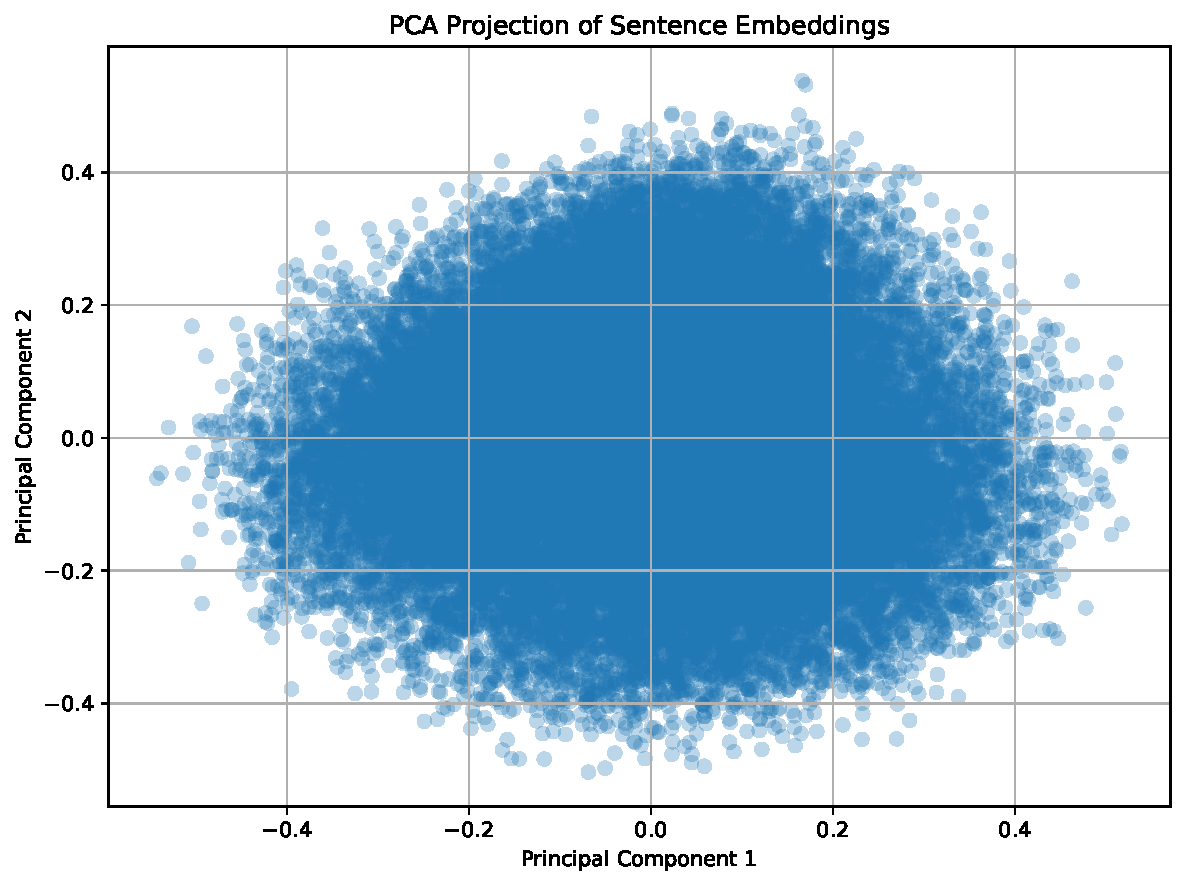
\includegraphics[keepaspectratio]{manifesto_text_clustering_files/figure-pdf/cell-19-output-2.pdf}}

To understand how the PCA dimensions relate to the underlying CMP
topics, we can color the points by the manually annotated categories.

\pandocbounded{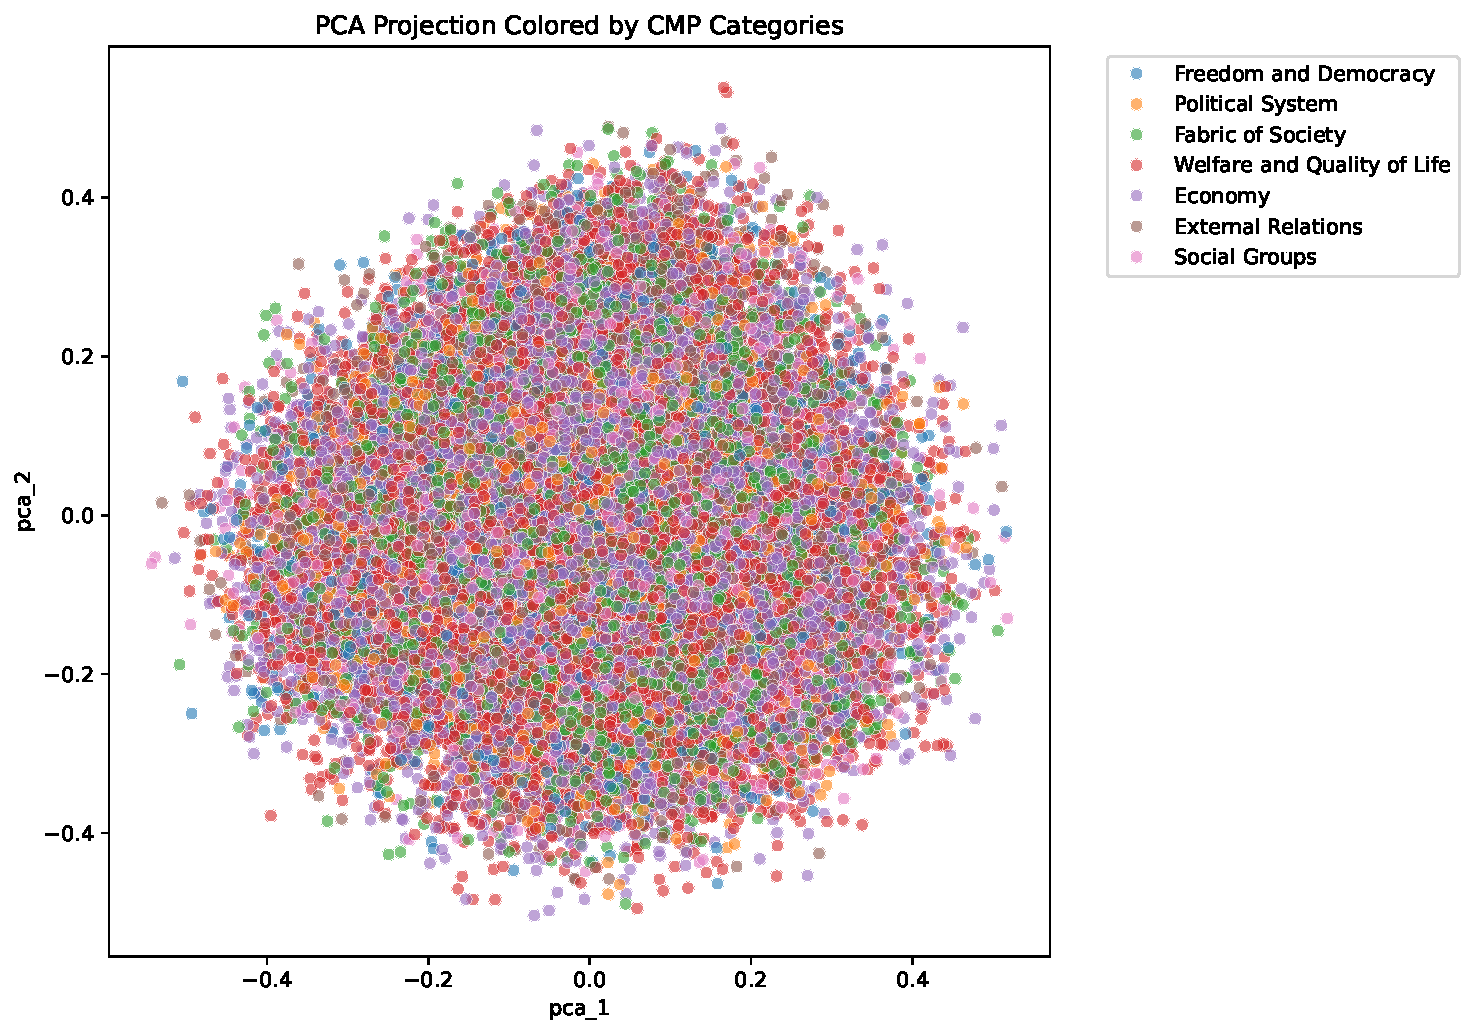
\includegraphics[keepaspectratio]{manifesto_text_clustering_files/figure-pdf/cell-20-output-1.pdf}}

The visualization shows some topic separation, although there is
noticeable overlap --- expected given the complexity and brevity of the
quasi-sentences.

\subsection{Clustering and Evaluation}\label{clustering-and-evaluation}

We apply two clustering algorithms: \textbf{k-means} and
\textbf{hierarchical agglomerative clustering} (Ward linkage). Since we
are working toward seven CMP topics, we set the number of clusters to
\texttt{k\ =\ 7}.

\subsubsection{K-Means Clustering}\label{k-means-clustering-1}

Evaluate clustering using Adjusted Rand Index (ARI), which measures
similarity between the clustering and the known \texttt{category} labels
(ignoring label names).

\begin{verbatim}
K-Means-Clustering aus Cache geladen.
Adjusted Rand Index (K-Means): 0.070
\end{verbatim}

\subsubsection{Hierarchical Clustering}\label{hierarchical-clustering}

\begin{verbatim}
Hierarchical Clustering aus Cache geladen.
Adjusted Rand Index (Hierarchical): 0.074
\end{verbatim}

\subsubsection{Cluster Composition and Topic
Alignment}\label{cluster-composition-and-topic-alignment}

To better understand what each cluster contains, we look at
representative sentences closest to the cluster centroids.

\begin{verbatim}
Cluster 0 Representative:
The reasons for this disadvantage may vary; but pension fund contributions, which increase with aging, are undoubtedly partly to blame.
--------------------------------------------------------------------------------
Cluster 1 Representative:
We will increasingly integrate preventive controls into antitrust law.
--------------------------------------------------------------------------------
Cluster 2 Representative:
Minimum sentences of ten years for sexual offenses
--------------------------------------------------------------------------------
Cluster 3 Representative:
We cannot predict what leeway the state will have after Corona.
--------------------------------------------------------------------------------
Cluster 4 Representative:
We have to do everything we can to keep it that way.
--------------------------------------------------------------------------------
Cluster 5 Representative:
The passenger car toll was a disaster waiting to happen.
--------------------------------------------------------------------------------
Cluster 6 Representative:
Extending political rights to all residents
--------------------------------------------------------------------------------
\end{verbatim}

This reveals interpretable topics per cluster, which are manually
compared to the seven CMP categories for qualitative alignment.

Cluster 0 = Cluster 1 = Cluster 2 = Cluster 3 = Cluster 4 = Cluster 5 =
Cluster 6 =


\printbibliography



\end{document}
